\documentclass[12pt]{article}
\usepackage{../../../format}
\lhead{A Level Physics - Turning Points}

\begin{document}
\begin{center}
\underline{\huge Special Relativity}
\end{center}
\section{Frames of reference}
Einstein's theory of special relativity is the result of analysing the consequences of the absence of any universal frame of reference. Special relativity concentrates on frames of reference which are moving at a constant velocity relative to each other. These frames are known as \textbf{inertial frames of reference}.\\
\\
Special relativity is based on two postulates:
\begin{itemize}
\item The laws of physics, expressed in equations, have the same form in all inertial frames
\item The speed of light in free space is invariant (ie the same for all observers regardless of their state of motion and the speed of the light source)
\end{itemize}
\section{The Michelson-Morley experiment}
The experiment was carried out to find out if the direction of the Earth's motion through space differs from the speed of light in a perpendicular direction. This was investigated using the Michelson interferometer, shown below:\\
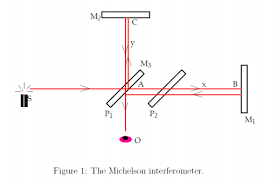
\includegraphics[width=10cm]{michelson.png}\\
The semi-silvered glass block splits the beam of monochromatic light into two beams at A which is on the silvered side of the block. The block, $P_2$, is necessary to ensure that both beams pass through the same thickness of glass and air. If the speed of light depended on the angle compared to the earth's rotation there would be interference at O due to the waves no longer being in phase. However this was not detected, meaning there is no difference in speed.
\section{Time dilation and proper time}
A consequence of the invariance of the speed of light in free space is that time runs slower when in motion. \\
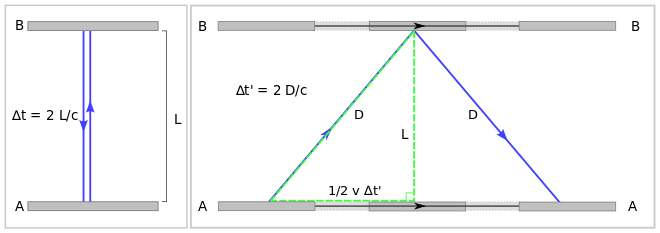
\includegraphics[width=8cm]{time_dilation.png}\\
This shows that to an observer time is slower to an observer.\\
\\
$$t=\frac{t_0}{\sqrt{1-(\frac{v}{c})^2}}$$
t- Time measured by external observer\\
$t_0$ - Time measured in the moving frame (called the proper time)\\
v - Relative velocity of moving frame\\
c- Speed of light in a vacuum
\subsection{Example experiment}
When cosmic rays reach the ionosphere above the Earth's surface, unstable sub-atomic particles called muons are created, travelling at 0.966c. These particles have a half life of $1.5\mu s$.\\
\\
Measurements by Bruno Rossi showed that about 80\% of the muons created by cosmic radiation on a mountain top reached an observatory 2km below. In one half-life of $1.5\mu s$, muons moving at 0.996c would decay, resulting in fewer detected at the bottom than the top.
\section{Length contraction}
A moving observer sees an object to appear smaller than it is (as measured in the stationary frame).\\
\\
Time contraction is \textbf{only} along the direction of travel.\\
It s easier to think that a moving observer measures the distance they cover to be less than a stationary observer.
$$L=L_0\sqrt{1-(\frac{v}{c})^2}$$
L - Length measured by the moving observer\\
$L_0$ - Length measured by the stationary observer (called the proper length)\\
v- Relative velocity of the moving frame\\
c- Speed of light in a vacuum
\section{Relativistic mass, momentum and energy}
\subsection{Relativistic mass}
Rest mass (proper mass,$m_0$):Mass as measured by an observer who is stationary relative to the mass\\
Relative mass(m): The apparent mass of an object that is moving relative to the observer (speed v)\\
$$m=\frac{m_0}{\sqrt{1-(\frac{v}{c})^2}}$$
Relativistic mass increases with speed
\newpage
\subsection{Relativistic momentum}
$$p=mv-\frac{m_0v}{\sqrt{1-(\frac{v}{c})^2}}$$
\subsection{Relativistic energy}
$$E=mc^2=\frac{m_0c^2}{\sqrt{1-(\frac{v}{c})^2}}$$
\subsubsection{Kinetic energy}
\begin{center}
Total energy=Rest energy+Relativistic KE
\end{center}
$$E=E_0+E_K$$
$$E_K=E-E_0$$
$$E_K=\frac{m_0c^2}{\sqrt{1-(\frac{v}{c})^2}}-m_0c^2$$
$$E_K=m_0c^2\Bigg(\bigg(1-\bigg(\frac{v}{c}\bigg)^2\bigg)^{-\frac{1}{2}}-1\Bigg)$$
\textcolor{red}{Apply binomial expansion to the first term}
$$E_K=m_0c^2\Bigg(1+\frac{1}{2}\Big(\frac{v}{c}\Big)^2+\frac{-\frac{1}{2}(-\frac{1}{2}-1)}{2}\times\Big(\frac{v}{c}\Big)^4-1\Bigg)$$
\textcolor{red}{Approximate away all terms larger than $\Big(\frac{v}{c}\Big)^2$ and simplify}
$$E_K\approx m_0c^2\times\frac{1}{2}\times\frac{v^2}{c^2}=\frac{1}{2}m_0v^2$$
Together mass and energy are conserved, but not necessaries individually
\section{Summary of equations}
{\renewcommand{\arraystretch}{2}
\begin{tabular}{l l}
Gamma factor&$\gamma=\sqrt{1-(\frac{v}{c})^2}$\\
Length contraction&$L_0\gamma$\\
Time dilation&\Large{$\frac{t_0}{\gamma}$}\\
Relativistic mass&\Large{$\frac{m_0}{\gamma}$}\\
Relativistic momentum&\Large{$\frac{m_0v}{\gamma}$}\\
Relativistic energy&\Large{$\frac{m_0c^2}{\gamma}$}
\end{tabular}}
\end{document}